\documentclass[1p]{elsarticle_modified}
%\bibliographystyle{elsarticle-num}

%\usepackage[colorlinks]{hyperref}
%\usepackage{abbrmath_seonhwa} %\Abb, \Ascr, \Acal ,\Abf, \Afrak
\usepackage{amsfonts}
\usepackage{amssymb}
\usepackage{amsmath}
\usepackage{amsthm}
\usepackage{scalefnt}
\usepackage{amsbsy}
\usepackage{kotex}
\usepackage{caption}
\usepackage{subfig}
\usepackage{color}
\usepackage{graphicx}
\usepackage{xcolor} %% white, black, red, green, blue, cyan, magenta, yellow
\usepackage{float}
\usepackage{setspace}
\usepackage{hyperref}

\usepackage{tikz}
\usetikzlibrary{arrows}

\usepackage{multirow}
\usepackage{array} % fixed length table
\usepackage{hhline}

%%%%%%%%%%%%%%%%%%%%%
\makeatletter
\renewcommand*\env@matrix[1][\arraystretch]{%
	\edef\arraystretch{#1}%
	\hskip -\arraycolsep
	\let\@ifnextchar\new@ifnextchar
	\array{*\c@MaxMatrixCols c}}
\makeatother %https://tex.stackexchange.com/questions/14071/how-can-i-increase-the-line-spacing-in-a-matrix
%%%%%%%%%%%%%%%

\usepackage[normalem]{ulem}

\newcommand{\msout}[1]{\ifmmode\text{\sout{\ensuremath{#1}}}\else\sout{#1}\fi}
%SOURCE: \msout is \stkout macro in https://tex.stackexchange.com/questions/20609/strikeout-in-math-mode

\newcommand{\cancel}[1]{
	\ifmmode
	{\color{red}\msout{#1}}
	\else
	{\color{red}\sout{#1}}
	\fi
}

\newcommand{\add}[1]{
	{\color{blue}\uwave{#1}}
}

\newcommand{\replace}[2]{
	\ifmmode
	{\color{red}\msout{#1}}{\color{blue}\uwave{#2}}
	\else
	{\color{red}\sout{#1}}{\color{blue}\uwave{#2}}
	\fi
}

\newcommand{\Sol}{\mathcal{S}} %segment
\newcommand{\D}{D} %diagram
\newcommand{\A}{\mathcal{A}} %arc


%%%%%%%%%%%%%%%%%%%%%%%%%%%%%5 test

\def\sl{\operatorname{\textup{SL}}(2,\Cbb)}
\def\psl{\operatorname{\textup{PSL}}(2,\Cbb)}
\def\quan{\mkern 1mu \triangleright \mkern 1mu}

\theoremstyle{definition}
\newtheorem{thm}{Theorem}[section]
\newtheorem{prop}[thm]{Proposition}
\newtheorem{lem}[thm]{Lemma}
\newtheorem{ques}[thm]{Question}
\newtheorem{cor}[thm]{Corollary}
\newtheorem{defn}[thm]{Definition}
\newtheorem{exam}[thm]{Example}
\newtheorem{rmk}[thm]{Remark}
\newtheorem{alg}[thm]{Algorithm}

\newcommand{\I}{\sqrt{-1}}
\begin{document}

%\begin{frontmatter}
%
%\title{Boundary parabolic representations of knots up to 8 crossings}
%
%%% Group authors per affiliation:
%\author{Yunhi Cho} 
%\address{Department of Mathematics, University of Seoul, Seoul, Korea}
%\ead{yhcho@uos.ac.kr}
%
%
%\author{Seonhwa Kim} %\fnref{s_kim}}
%\address{Center for Geometry and Physics, Institute for Basic Science, Pohang, 37673, Korea}
%\ead{ryeona17@ibs.re.kr}
%
%\author{Hyuk Kim}
%\address{Department of Mathematical Sciences, Seoul National University, Seoul 08826, Korea}
%\ead{hyukkim@snu.ac.kr}
%
%\author{Seokbeom Yoon}
%\address{Department of Mathematical Sciences, Seoul National University, Seoul, 08826,  Korea}
%\ead{sbyoon15@snu.ac.kr}
%
%\begin{abstract}
%We find all boundary parabolic representation of knots up to 8 crossings.
%
%\end{abstract}
%\begin{keyword}
%    \MSC[2010] 57M25 
%\end{keyword}
%
%\end{frontmatter}

%\linenumbers
%\tableofcontents
%
\newcommand\colored[1]{\textcolor{white}{\rule[-0.35ex]{0.8em}{1.4ex}}\kern-0.8em\color{red} #1}%
%\newcommand\colored[1]{\textcolor{white}{ #1}\kern-2.17ex	\textcolor{white}{ #1}\kern-1.81ex	\textcolor{white}{ #1}\kern-2.15ex\color{red}#1	}

{\Large $\underline{12n_{0302}~(K12n_{0302})}$}

\setlength{\tabcolsep}{10pt}
\renewcommand{\arraystretch}{1.6}
\vspace{1cm}\begin{tabular}{m{100pt}>{\centering\arraybackslash}m{274pt}}
\multirow{5}{120pt}{
	\centering
	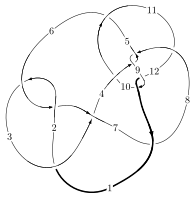
\includegraphics[width=112pt]{../../../GIT/diagram.site/Diagrams/png/2391_12n_0302.png}\\
\ \ \ A knot diagram\footnotemark}&
\allowdisplaybreaks
\textbf{Linearized knot diagam} \\
\cline{2-2}
 &
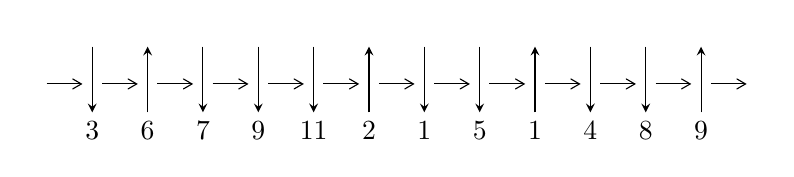
\begin{tikzpicture}[x=20pt, y=17pt]
	% nodes
	\node (C0) at (0, 0) {};
	\node (C1) at (1, 0) {};
	\node (C1U) at (1, +1) {};
	\node (C1D) at (1, -1) {3};

	\node (C2) at (2, 0) {};
	\node (C2U) at (2, +1) {};
	\node (C2D) at (2, -1) {6};

	\node (C3) at (3, 0) {};
	\node (C3U) at (3, +1) {};
	\node (C3D) at (3, -1) {7};

	\node (C4) at (4, 0) {};
	\node (C4U) at (4, +1) {};
	\node (C4D) at (4, -1) {9};

	\node (C5) at (5, 0) {};
	\node (C5U) at (5, +1) {};
	\node (C5D) at (5, -1) {11};

	\node (C6) at (6, 0) {};
	\node (C6U) at (6, +1) {};
	\node (C6D) at (6, -1) {2};

	\node (C7) at (7, 0) {};
	\node (C7U) at (7, +1) {};
	\node (C7D) at (7, -1) {1};

	\node (C8) at (8, 0) {};
	\node (C8U) at (8, +1) {};
	\node (C8D) at (8, -1) {5};

	\node (C9) at (9, 0) {};
	\node (C9U) at (9, +1) {};
	\node (C9D) at (9, -1) {1};

	\node (C10) at (10, 0) {};
	\node (C10U) at (10, +1) {};
	\node (C10D) at (10, -1) {4};

	\node (C11) at (11, 0) {};
	\node (C11U) at (11, +1) {};
	\node (C11D) at (11, -1) {8};

	\node (C12) at (12, 0) {};
	\node (C12U) at (12, +1) {};
	\node (C12D) at (12, -1) {9};
	\node (C13) at (13, 0) {};

	% arrows
	\draw[->,>={angle 60}]
	(C0) edge (C1) (C1) edge (C2) (C2) edge (C3) (C3) edge (C4) (C4) edge (C5) (C5) edge (C6) (C6) edge (C7) (C7) edge (C8) (C8) edge (C9) (C9) edge (C10) (C10) edge (C11) (C11) edge (C12) (C12) edge (C13) ;	\draw[->,>=stealth]
	(C1U) edge (C1D) (C2D) edge (C2U) (C3U) edge (C3D) (C4U) edge (C4D) (C5U) edge (C5D) (C6D) edge (C6U) (C7U) edge (C7D) (C8U) edge (C8D) (C9D) edge (C9U) (C10U) edge (C10D) (C11U) edge (C11D) (C12D) edge (C12U) ;
	\end{tikzpicture} \\
\hhline{~~} \\& 
\textbf{Solving Sequence} \\ \cline{2-2} 
 &
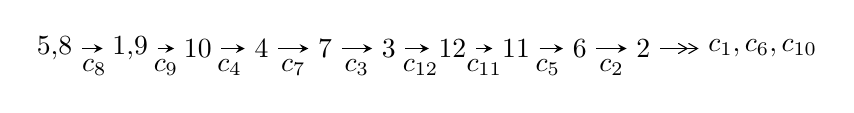
\begin{tikzpicture}[x=23pt, y=7pt]
	% node
	\node (A0) at (-1/8, 0) {5,8};
	\node (A1) at (17/16, 0) {1,9};
	\node (A2) at (17/8, 0) {10};
	\node (A3) at (25/8, 0) {4};
	\node (A4) at (33/8, 0) {7};
	\node (A5) at (41/8, 0) {3};
	\node (A6) at (49/8, 0) {12};
	\node (A7) at (57/8, 0) {11};
	\node (A8) at (65/8, 0) {6};
	\node (A9) at (73/8, 0) {2};
	\node (C1) at (1/2, -1) {$c_{8}$};
	\node (C2) at (13/8, -1) {$c_{9}$};
	\node (C3) at (21/8, -1) {$c_{4}$};
	\node (C4) at (29/8, -1) {$c_{7}$};
	\node (C5) at (37/8, -1) {$c_{3}$};
	\node (C6) at (45/8, -1) {$c_{12}$};
	\node (C7) at (53/8, -1) {$c_{11}$};
	\node (C8) at (61/8, -1) {$c_{5}$};
	\node (C9) at (69/8, -1) {$c_{2}$};
	\node (A10) at (11, 0) {$c_{1},c_{6},c_{10}$};

	% edge
	\draw[->,>=stealth]	
	(A0) edge (A1) (A1) edge (A2) (A2) edge (A3) (A3) edge (A4) (A4) edge (A5) (A5) edge (A6) (A6) edge (A7) (A7) edge (A8) (A8) edge (A9) ;
	\draw[->>,>={angle 60}]	
	(A9) edge (A10);
\end{tikzpicture} \\ 

\end{tabular} \\

\footnotetext{
The image of knot diagram is generated by the software ``\textbf{Draw programme}" developed by Andrew Bartholomew(\url{http://www.layer8.co.uk/maths/draw/index.htm\#Running-draw}), where we modified some parts for our purpose(\url{https://github.com/CATsTAILs/LinksPainter}).
}\phantom \\ \newline 
\centering \textbf{Ideals for irreducible components\footnotemark of $X_{\text{par}}$} 
 
\begin{align*}
I^u_{1}&=\langle 
- u^{30}- u^{29}+\cdots+64 b+1,\;u^{30}+u^{29}+\cdots+64 a-65,\;u^{31}+4 u^{29}+\cdots+2 u-1\rangle \\
I^u_{2}&=\langle 
1.68907\times10^{23} u^{35}-1.11374\times10^{23} u^{34}+\cdots+9.33256\times10^{23} b+1.62659\times10^{24},\\
\phantom{I^u_{2}}&\phantom{= \langle  }-2.83334\times10^{24} u^{35}+1.80304\times10^{24} u^{34}+\cdots+1.58653\times10^{25} a+2.57411\times10^{25},\\
\phantom{I^u_{2}}&\phantom{= \langle  }u^{36}- u^{35}+\cdots-44 u+17\rangle \\
I^u_{3}&=\langle 
b+a+1,\;a^6+a^5 u+6 a^5+5 a^4 u+16 a^4+12 a^3 u+24 a^3+16 a^2 u+21 a^2+12 a u+10 a+4 u+1,\;u^2+1\rangle \\
\\
\end{align*}
\raggedright * 3 irreducible components of $\dim_{\mathbb{C}}=0$, with total 79 representations.\\
\footnotetext{All coefficients of polynomials are rational numbers. But the coefficients are sometimes approximated in decimal forms when there is not enough margin.}
\newpage
\renewcommand{\arraystretch}{1}
\centering \section*{I. $I^u_{1}= \langle - u^{30}- u^{29}+\cdots+64 b+1,\;u^{30}+u^{29}+\cdots+64 a-65,\;u^{31}+4 u^{29}+\cdots+2 u-1 \rangle$}
\flushleft \textbf{(i) Arc colorings}\\
\begin{tabular}{m{7pt} m{180pt} m{7pt} m{180pt} }
\flushright $a_{5}=$&$\begin{pmatrix}0\\u\end{pmatrix}$ \\
\flushright $a_{8}=$&$\begin{pmatrix}1\\0\end{pmatrix}$ \\
\flushright $a_{1}=$&$\begin{pmatrix}-0.0156250 u^{30}-0.0156250 u^{29}+\cdots-0.0156250 u+1.01563\\0.0156250 u^{30}+0.0156250 u^{29}+\cdots+0.0156250 u-0.0156250\end{pmatrix}$ \\
\flushright $a_{9}=$&$\begin{pmatrix}1\\u^2\end{pmatrix}$ \\
\flushright $a_{10}=$&$\begin{pmatrix}-0.0156250 u^{30}-0.0156250 u^{29}+\cdots-0.0156250 u+1.01563\\0.0156250 u^{30}+0.0156250 u^{29}+\cdots+0.0156250 u-0.0156250\end{pmatrix}$ \\
\flushright $a_{4}=$&$\begin{pmatrix}u\\u^3+u\end{pmatrix}$ \\
\flushright $a_{7}=$&$\begin{pmatrix}-0.171875 u^{30}-0.203125 u^{29}+\cdots-0.265625 u+1.23438\\\frac{5}{32} u^{30}+\frac{3}{16} u^{29}+\cdots+\frac{1}{4} u-\frac{7}{32}\end{pmatrix}$ \\
\flushright $a_{3}=$&$\begin{pmatrix}-2.37500 u^{30}-0.125000 u^{29}+\cdots+7.68750 u-0.625000\\1.45313 u^{30}+0.453125 u^{29}+\cdots-2.23438 u+0.0468750\end{pmatrix}$ \\
\flushright $a_{12}=$&$\begin{pmatrix}-0.0156250 u^{30}-0.0156250 u^{29}+\cdots-0.0156250 u+1.01563\\0.0156250 u^{30}+0.0156250 u^{29}+\cdots+0.0156250 u-0.0156250\end{pmatrix}$ \\
\flushright $a_{11}=$&$\begin{pmatrix}1\\0.0156250 u^{30}+0.0156250 u^{29}+\cdots+0.0156250 u-0.0156250\end{pmatrix}$ \\
\flushright $a_{6}=$&$\begin{pmatrix}- u\\-0.0156250 u^{30}+0.0156250 u^{29}+\cdots+1.04688 u-0.0156250\end{pmatrix}$ \\
\flushright $a_{2}=$&$\begin{pmatrix}-2.45313 u^{30}-1.10938 u^{29}+\cdots+6.73438 u+1.04688\\\frac{1}{32} u^{30}+\frac{43}{32} u^{29}+\cdots+\frac{61}{16} u-\frac{7}{2}\end{pmatrix}$\\&\end{tabular}
\flushleft \textbf{(ii) Obstruction class $= -1$}\\~\\
\flushleft \textbf{(iii) Cusp Shapes $= -\frac{15}{8} u^{30}+\frac{7}{2} u^{29}+\cdots+\frac{343}{16} u-\frac{181}{16}$}\\~\\
\newpage\renewcommand{\arraystretch}{1}
\flushleft \textbf{(iv) u-Polynomials at the component}\newline \\
\begin{tabular}{m{50pt}|m{274pt}}
Crossings & \hspace{64pt}u-Polynomials at each crossing \\
\hline $$\begin{aligned}c_{1}\end{aligned}$$&$\begin{aligned}
&u^{31}+15 u^{30}+\cdots-3 u-4
\end{aligned}$\\
\hline $$\begin{aligned}c_{2},c_{6}\end{aligned}$$&$\begin{aligned}
&u^{31}-3 u^{30}+\cdots-5 u+2
\end{aligned}$\\
\hline $$\begin{aligned}c_{3}\end{aligned}$$&$\begin{aligned}
&u^{31}+3 u^{30}+\cdots-13 u+2
\end{aligned}$\\
\hline $$\begin{aligned}c_{4},c_{5},c_{8}\end{aligned}$$&$\begin{aligned}
&u^{31}+4 u^{29}+\cdots+2 u+1
\end{aligned}$\\
\hline $$\begin{aligned}c_{7}\end{aligned}$$&$\begin{aligned}
&u^{31}-15 u^{30}+\cdots-971 u+86
\end{aligned}$\\
\hline $$\begin{aligned}c_{9},c_{12}\end{aligned}$$&$\begin{aligned}
&u^{31}-8 u^{30}+\cdots-12 u+1
\end{aligned}$\\
\hline $$\begin{aligned}c_{10}\end{aligned}$$&$\begin{aligned}
&u^{31}-19 u^{29}+\cdots+328 u+73
\end{aligned}$\\
\hline $$\begin{aligned}c_{11}\end{aligned}$$&$\begin{aligned}
&u^{31}+29 u^{30}+\cdots+2490368 u+262144
\end{aligned}$\\
\hline
\end{tabular}\\~\\
\newpage\renewcommand{\arraystretch}{1}
\flushleft \textbf{(v) Riley Polynomials at the component}\newline \\
\begin{tabular}{m{50pt}|m{274pt}}
Crossings & \hspace{64pt}Riley Polynomials at each crossing \\
\hline $$\begin{aligned}c_{1}\end{aligned}$$&$\begin{aligned}
&y^{31}+3 y^{30}+\cdots+129 y-16
\end{aligned}$\\
\hline $$\begin{aligned}c_{2},c_{6}\end{aligned}$$&$\begin{aligned}
&y^{31}+15 y^{30}+\cdots-3 y-4
\end{aligned}$\\
\hline $$\begin{aligned}c_{3}\end{aligned}$$&$\begin{aligned}
&y^{31}-9 y^{30}+\cdots-27 y-4
\end{aligned}$\\
\hline $$\begin{aligned}c_{4},c_{5},c_{8}\end{aligned}$$&$\begin{aligned}
&y^{31}+8 y^{30}+\cdots-12 y-1
\end{aligned}$\\
\hline $$\begin{aligned}c_{7}\end{aligned}$$&$\begin{aligned}
&y^{31}+3 y^{30}+\cdots+25565 y-7396
\end{aligned}$\\
\hline $$\begin{aligned}c_{9},c_{12}\end{aligned}$$&$\begin{aligned}
&y^{31}+44 y^{30}+\cdots+4 y-1
\end{aligned}$\\
\hline $$\begin{aligned}c_{10}\end{aligned}$$&$\begin{aligned}
&y^{31}-38 y^{30}+\cdots+121892 y-5329
\end{aligned}$\\
\hline $$\begin{aligned}c_{11}\end{aligned}$$&$\begin{aligned}
&y^{31}-7 y^{30}+\cdots+188978561024 y-68719476736
\end{aligned}$\\
\hline
\end{tabular}\\~\\
\newpage\flushleft \textbf{(vi) Complex Volumes and Cusp Shapes}
$$\begin{array}{c|c|c}  
\text{Solutions to }I^u_{1}& \I (\text{vol} + \sqrt{-1}CS) & \text{Cusp shape}\\
 \hline 
\begin{aligned}
u &= \phantom{-}0.428614 + 0.787639 I \\
a &= \phantom{-}0.020444 - 1.071240 I \\
b &= \phantom{-}0.277691 + 1.156760 I\end{aligned}
 & \phantom{-}2.11446 - 7.62347 I & -2.55486 + 10.23287 I \\ \hline\begin{aligned}
u &= \phantom{-}0.428614 - 0.787639 I \\
a &= \phantom{-}0.020444 + 1.071240 I \\
b &= \phantom{-}0.277691 - 1.156760 I\end{aligned}
 & \phantom{-}2.11446 + 7.62347 I & -2.55486 - 10.23287 I \\ \hline\begin{aligned}
u &= -0.398489 + 0.747920 I \\
a &= \phantom{-}0.277025 + 1.072210 I \\
b &= \phantom{-}0.127552 - 1.190720 I\end{aligned}
 & \phantom{-}3.81643 + 2.62838 I & \phantom{-}0.13136 - 5.27727 I \\ \hline\begin{aligned}
u &= -0.398489 - 0.747920 I \\
a &= \phantom{-}0.277025 - 1.072210 I \\
b &= \phantom{-}0.127552 + 1.190720 I\end{aligned}
 & \phantom{-}3.81643 - 2.62838 I & \phantom{-}0.13136 + 5.27727 I \\ \hline\begin{aligned}
u &= -0.823498 + 0.113059 I \\
a &= \phantom{-}0.851475 - 0.053587 I \\
b &= \phantom{-}1.221930 - 0.380414 I\end{aligned}
 & -4.06065 + 3.78130 I & -10.92047 - 4.50880 I \\ \hline\begin{aligned}
u &= -0.823498 - 0.113059 I \\
a &= \phantom{-}0.851475 + 0.053587 I \\
b &= \phantom{-}1.221930 + 0.380414 I\end{aligned}
 & -4.06065 - 3.78130 I & -10.92047 + 4.50880 I \\ \hline\begin{aligned}
u &= -0.308639 + 0.692422 I \\
a &= \phantom{-}0.807667 + 1.093890 I \\
b &= -0.226940 - 1.192890 I\end{aligned}
 & \phantom{-}3.71218 + 0.23183 I & -0.44077 - 4.37023 I \\ \hline\begin{aligned}
u &= -0.308639 - 0.692422 I \\
a &= \phantom{-}0.807667 - 1.093890 I \\
b &= -0.226940 + 1.192890 I\end{aligned}
 & \phantom{-}3.71218 - 0.23183 I & -0.44077 + 4.37023 I \\ \hline\begin{aligned}
u &= \phantom{-}0.737257 + 0.999674 I \\
a &= -1.014960 + 0.279964 I \\
b &= -0.405856 - 0.149663 I\end{aligned}
 & -1.01582 - 3.41753 I & -1.81646 + 1.83833 I \\ \hline\begin{aligned}
u &= \phantom{-}0.737257 - 0.999674 I \\
a &= -1.014960 - 0.279964 I \\
b &= -0.405856 + 0.149663 I\end{aligned}
 & -1.01582 + 3.41753 I & -1.81646 - 1.83833 I\\
 \hline 
 \end{array}$$\newpage$$\begin{array}{c|c|c}  
\text{Solutions to }I^u_{1}& \I (\text{vol} + \sqrt{-1}CS) & \text{Cusp shape}\\
 \hline 
\begin{aligned}
u &= \phantom{-}0.493312 + 0.567058 I \\
a &= \phantom{-}0.507385 - 0.402871 I \\
b &= \phantom{-}0.107522 + 0.874845 I\end{aligned}
 & -0.97829 - 1.43223 I & -7.64253 + 4.49429 I \\ \hline\begin{aligned}
u &= \phantom{-}0.493312 - 0.567058 I \\
a &= \phantom{-}0.507385 + 0.402871 I \\
b &= \phantom{-}0.107522 - 0.874845 I\end{aligned}
 & -0.97829 + 1.43223 I & -7.64253 - 4.49429 I \\ \hline\begin{aligned}
u &= \phantom{-}0.263305 + 0.688070 I \\
a &= \phantom{-}1.04620 - 1.12763 I \\
b &= -0.418303 + 1.197120 I\end{aligned}
 & \phantom{-}1.88939 + 4.73630 I & -3.89657 - 0.59420 I \\ \hline\begin{aligned}
u &= \phantom{-}0.263305 - 0.688070 I \\
a &= \phantom{-}1.04620 + 1.12763 I \\
b &= -0.418303 - 1.197120 I\end{aligned}
 & \phantom{-}1.88939 - 4.73630 I & -3.89657 + 0.59420 I \\ \hline\begin{aligned}
u &= \phantom{-}0.896581 + 0.914182 I \\
a &= -0.497658 + 0.734722 I \\
b &= -1.22042 + 0.80006 I\end{aligned}
 & -4.16004 - 2.58701 I & -4.00000 + 2.53611 I \\ \hline\begin{aligned}
u &= \phantom{-}0.896581 - 0.914182 I \\
a &= -0.497658 - 0.734722 I \\
b &= -1.22042 - 0.80006 I\end{aligned}
 & -4.16004 + 2.58701 I & -4.00000 - 2.53611 I \\ \hline\begin{aligned}
u &= -0.747911 + 1.060550 I \\
a &= -1.244110 - 0.413683 I \\
b &= -0.518247 + 0.621142 I\end{aligned}
 & -0.50947 + 8.32474 I & -0.66671 - 7.63696 I \\ \hline\begin{aligned}
u &= -0.747911 - 1.060550 I \\
a &= -1.244110 + 0.413683 I \\
b &= -0.518247 - 0.621142 I\end{aligned}
 & -0.50947 - 8.32474 I & -0.66671 + 7.63696 I \\ \hline\begin{aligned}
u &= -0.946068 + 0.895466 I \\
a &= -0.369074 - 0.860893 I \\
b &= -1.39985 - 1.14923 I\end{aligned}
 & -6.97286 - 2.17567 I & -7.38278 + 1.16604 I \\ \hline\begin{aligned}
u &= -0.946068 - 0.895466 I \\
a &= -0.369074 + 0.860893 I \\
b &= -1.39985 + 1.14923 I\end{aligned}
 & -6.97286 + 2.17567 I & -7.38278 - 1.16604 I\\
 \hline 
 \end{array}$$\newpage$$\begin{array}{c|c|c}  
\text{Solutions to }I^u_{1}& \I (\text{vol} + \sqrt{-1}CS) & \text{Cusp shape}\\
 \hline 
\begin{aligned}
u &= -0.918427 + 0.979157 I \\
a &= -0.674803 - 0.903235 I \\
b &= -1.66201 - 0.48080 I\end{aligned}
 & -8.26580 + 6.12965 I & -8.72219 - 5.26564 I \\ \hline\begin{aligned}
u &= -0.918427 - 0.979157 I \\
a &= -0.674803 + 0.903235 I \\
b &= -1.66201 + 0.48080 I\end{aligned}
 & -8.26580 - 6.12965 I & -8.72219 + 5.26564 I \\ \hline\begin{aligned}
u &= \phantom{-}0.654707\phantom{ +0.000000I} \\
a &= \phantom{-}0.828573\phantom{ +0.000000I} \\
b &= \phantom{-}0.783801\phantom{ +0.000000I}\end{aligned}
 & -1.18982\phantom{ +0.000000I} & -8.14570\phantom{ +0.000000I} \\ \hline\begin{aligned}
u &= -0.789945 + 1.134080 I \\
a &= -1.45883 - 0.71380 I \\
b &= -0.97512 + 1.29471 I\end{aligned}
 & -2.55844 + 10.54750 I & -1.65094 - 6.34331 I \\ \hline\begin{aligned}
u &= -0.789945 - 1.134080 I \\
a &= -1.45883 + 0.71380 I \\
b &= -0.97512 - 1.29471 I\end{aligned}
 & -2.55844 - 10.54750 I & -1.65094 + 6.34331 I \\ \hline\begin{aligned}
u &= \phantom{-}0.831569 + 1.116210 I \\
a &= -1.30990 + 0.83774 I \\
b &= -1.38338 - 1.03976 I\end{aligned}
 & -7.22926 - 7.46449 I & -7.55894 + 4.20366 I \\ \hline\begin{aligned}
u &= \phantom{-}0.831569 - 1.116210 I \\
a &= -1.30990 - 0.83774 I \\
b &= -1.38338 + 1.03976 I\end{aligned}
 & -7.22926 + 7.46449 I & -7.55894 - 4.20366 I \\ \hline\begin{aligned}
u &= \phantom{-}0.796078 + 1.157720 I \\
a &= -1.53812 + 0.78506 I \\
b &= -1.06685 - 1.54659 I\end{aligned}
 & -5.0523 - 15.6504 I & -4.62054 + 9.85010 I \\ \hline\begin{aligned}
u &= \phantom{-}0.796078 - 1.157720 I \\
a &= -1.53812 - 0.78506 I \\
b &= -1.06685 + 1.54659 I\end{aligned}
 & -5.0523 + 15.6504 I & -4.62054 - 9.85010 I \\ \hline\begin{aligned}
u &= \phantom{-}0.158909 + 0.450532 I \\
a &= \phantom{-}1.182970 - 0.267894 I \\
b &= -0.349614 + 0.360185 I\end{aligned}
 & -0.56592 - 1.41483 I & -5.18401 + 4.52622 I\\
 \hline 
 \end{array}$$\newpage$$\begin{array}{c|c|c}  
\text{Solutions to }I^u_{1}& \I (\text{vol} + \sqrt{-1}CS) & \text{Cusp shape}\\
 \hline 
\begin{aligned}
u &= \phantom{-}0.158909 - 0.450532 I \\
a &= \phantom{-}1.182970 + 0.267894 I \\
b &= -0.349614 - 0.360185 I\end{aligned}
 & -0.56592 + 1.41483 I & -5.18401 - 4.52622 I\\
 \hline 
 \end{array}$$\newpage\newpage\renewcommand{\arraystretch}{1}
\centering \section*{II. $I^u_{2}= \langle 1.69\times10^{23} u^{35}-1.11\times10^{23} u^{34}+\cdots+9.33\times10^{23} b+1.63\times10^{24},\;-2.83\times10^{24} u^{35}+1.80\times10^{24} u^{34}+\cdots+1.59\times10^{25} a+2.57\times10^{25},\;u^{36}- u^{35}+\cdots-44 u+17 \rangle$}
\flushleft \textbf{(i) Arc colorings}\\
\begin{tabular}{m{7pt} m{180pt} m{7pt} m{180pt} }
\flushright $a_{5}=$&$\begin{pmatrix}0\\u\end{pmatrix}$ \\
\flushright $a_{8}=$&$\begin{pmatrix}1\\0\end{pmatrix}$ \\
\flushright $a_{1}=$&$\begin{pmatrix}0.178587 u^{35}-0.113646 u^{34}+\cdots-2.60843 u-1.62248\\-0.180987 u^{35}+0.119339 u^{34}+\cdots-0.246496 u-1.74292\end{pmatrix}$ \\
\flushright $a_{9}=$&$\begin{pmatrix}1\\u^2\end{pmatrix}$ \\
\flushright $a_{10}=$&$\begin{pmatrix}-0.00240038 u^{35}+0.00569313 u^{34}+\cdots-2.85493 u-2.36540\\0.0118866 u^{35}-0.0147001 u^{34}+\cdots-0.196623 u-1.07676\end{pmatrix}$ \\
\flushright $a_{4}=$&$\begin{pmatrix}u\\u^3+u\end{pmatrix}$ \\
\flushright $a_{7}=$&$\begin{pmatrix}0.116243 u^{35}-0.0798703 u^{34}+\cdots-2.42275 u-0.678453\\-0.208906 u^{35}+0.154096 u^{34}+\cdots-0.572363 u-1.69509\end{pmatrix}$ \\
\flushright $a_{3}=$&$\begin{pmatrix}0.0899876 u^{35}-0.234769 u^{34}+\cdots+6.71425 u-2.77653\\0.0464972 u^{35}-0.00440409 u^{34}+\cdots+2.00161 u-0.344605\end{pmatrix}$ \\
\flushright $a_{12}=$&$\begin{pmatrix}0.0509778 u^{35}-0.0297385 u^{34}+\cdots-2.54053 u-0.983544\\-1\end{pmatrix}$ \\
\flushright $a_{11}=$&$\begin{pmatrix}0.0509778 u^{35}-0.0297385 u^{34}+\cdots-2.54053 u-1.98354\\-1\end{pmatrix}$ \\
\flushright $a_{6}=$&$\begin{pmatrix}-0.0375842 u^{35}-0.0900247 u^{34}+\cdots-7.79934 u+1.72161\\0.0212393 u^{35}-0.148848 u^{34}+\cdots+1.25948 u-0.866623\end{pmatrix}$ \\
\flushright $a_{2}=$&$\begin{pmatrix}0.267879 u^{35}-0.421650 u^{34}+\cdots+20.4123 u-11.1581\\0.0138355 u^{35}+0.221537 u^{34}+\cdots+0.400166 u-0.936209\end{pmatrix}$\\&\end{tabular}
\flushleft \textbf{(ii) Obstruction class $= -1$}\\~\\
\flushleft \textbf{(iii) Cusp Shapes $= -\frac{94459427649077696837288}{933255522779965433376737} u^{35}+\frac{1669130199746521433848712}{933255522779965433376737} u^{34}+\cdots-\frac{25170861470598659641440976}{933255522779965433376737} u+\frac{1667795781533429661370718}{933255522779965433376737}$}\\~\\
\newpage\renewcommand{\arraystretch}{1}
\flushleft \textbf{(iv) u-Polynomials at the component}\newline \\
\begin{tabular}{m{50pt}|m{274pt}}
Crossings & \hspace{64pt}u-Polynomials at each crossing \\
\hline $$\begin{aligned}c_{1}\end{aligned}$$&$\begin{aligned}
&(u^{18}+9 u^{17}+\cdots+u+1)^{2}
\end{aligned}$\\
\hline $$\begin{aligned}c_{2},c_{6}\end{aligned}$$&$\begin{aligned}
&(u^{18}+u^{17}+\cdots+u+1)^{2}
\end{aligned}$\\
\hline $$\begin{aligned}c_{3}\end{aligned}$$&$\begin{aligned}
&(u^{18}- u^{17}+\cdots- u+5)^{2}
\end{aligned}$\\
\hline $$\begin{aligned}c_{4},c_{5},c_{8}\end{aligned}$$&$\begin{aligned}
&u^{36}+u^{35}+\cdots+44 u+17
\end{aligned}$\\
\hline $$\begin{aligned}c_{7}\end{aligned}$$&$\begin{aligned}
&(u^{18}+5 u^{17}+\cdots+13 u+3)^{2}
\end{aligned}$\\
\hline $$\begin{aligned}c_{9},c_{12}\end{aligned}$$&$\begin{aligned}
&u^{36}-15 u^{35}+\cdots-3300 u+289
\end{aligned}$\\
\hline $$\begin{aligned}c_{10}\end{aligned}$$&$\begin{aligned}
&u^{36}+u^{35}+\cdots-22616 u+236209
\end{aligned}$\\
\hline $$\begin{aligned}c_{11}\end{aligned}$$&$\begin{aligned}
&(u-1)^{36}
\end{aligned}$\\
\hline
\end{tabular}\\~\\
\newpage\renewcommand{\arraystretch}{1}
\flushleft \textbf{(v) Riley Polynomials at the component}\newline \\
\begin{tabular}{m{50pt}|m{274pt}}
Crossings & \hspace{64pt}Riley Polynomials at each crossing \\
\hline $$\begin{aligned}c_{1}\end{aligned}$$&$\begin{aligned}
&(y^{18}+y^{17}+\cdots+9 y+1)^{2}
\end{aligned}$\\
\hline $$\begin{aligned}c_{2},c_{6}\end{aligned}$$&$\begin{aligned}
&(y^{18}+9 y^{17}+\cdots+y+1)^{2}
\end{aligned}$\\
\hline $$\begin{aligned}c_{3}\end{aligned}$$&$\begin{aligned}
&(y^{18}-7 y^{17}+\cdots-91 y+25)^{2}
\end{aligned}$\\
\hline $$\begin{aligned}c_{4},c_{5},c_{8}\end{aligned}$$&$\begin{aligned}
&y^{36}+15 y^{35}+\cdots+3300 y+289
\end{aligned}$\\
\hline $$\begin{aligned}c_{7}\end{aligned}$$&$\begin{aligned}
&(y^{18}-3 y^{17}+\cdots+5 y+9)^{2}
\end{aligned}$\\
\hline $$\begin{aligned}c_{9},c_{12}\end{aligned}$$&$\begin{aligned}
&y^{36}+11 y^{35}+\cdots+3006276 y+83521
\end{aligned}$\\
\hline $$\begin{aligned}c_{10}\end{aligned}$$&$\begin{aligned}
&y^{36}-5 y^{35}+\cdots-292100155924 y+55794691681
\end{aligned}$\\
\hline $$\begin{aligned}c_{11}\end{aligned}$$&$\begin{aligned}
&(y-1)^{36}
\end{aligned}$\\
\hline
\end{tabular}\\~\\
\newpage\flushleft \textbf{(vi) Complex Volumes and Cusp Shapes}
$$\begin{array}{c|c|c}  
\text{Solutions to }I^u_{2}& \I (\text{vol} + \sqrt{-1}CS) & \text{Cusp shape}\\
 \hline 
\begin{aligned}
u &= -0.320634 + 0.870916 I \\
a &= -1.59556 + 0.83474 I \\
b &= \phantom{-}0.087095 + 0.616918 I\end{aligned}
 & \phantom{-}4.20760 + 0.97328 I & \phantom{-}2.11395 - 4.55184 I \\ \hline\begin{aligned}
u &= -0.320634 - 0.870916 I \\
a &= -1.59556 - 0.83474 I \\
b &= \phantom{-}0.087095 - 0.616918 I\end{aligned}
 & \phantom{-}4.20760 - 0.97328 I & \phantom{-}2.11395 + 4.55184 I \\ \hline\begin{aligned}
u &= -0.828905 + 0.682944 I \\
a &= \phantom{-}0.886516 + 0.217948 I \\
b &= \phantom{-}0.420070 + 0.303007 I\end{aligned}
 & -1.65768 - 2.36433 I & -3.03894 + 3.34702 I \\ \hline\begin{aligned}
u &= -0.828905 - 0.682944 I \\
a &= \phantom{-}0.886516 - 0.217948 I \\
b &= \phantom{-}0.420070 - 0.303007 I\end{aligned}
 & -1.65768 + 2.36433 I & -3.03894 - 3.34702 I \\ \hline\begin{aligned}
u &= \phantom{-}0.338195 + 1.021420 I \\
a &= -1.33297 - 1.04821 I \\
b &= \phantom{-}0.609948 - 0.458991 I\end{aligned}
 & \phantom{-}2.68166 + 3.09151 I & -0.88507 - 2.77317 I \\ \hline\begin{aligned}
u &= \phantom{-}0.338195 - 1.021420 I \\
a &= -1.33297 + 1.04821 I \\
b &= \phantom{-}0.609948 + 0.458991 I\end{aligned}
 & \phantom{-}2.68166 - 3.09151 I & -0.88507 + 2.77317 I \\ \hline\begin{aligned}
u &= \phantom{-}0.786288 + 0.800353 I \\
a &= \phantom{-}1.137130 - 0.178590 I \\
b &= \phantom{-}0.420070 + 0.303007 I\end{aligned}
 & -1.65768 - 2.36433 I & -3.03894 + 3.34702 I \\ \hline\begin{aligned}
u &= \phantom{-}0.786288 - 0.800353 I \\
a &= \phantom{-}1.137130 + 0.178590 I \\
b &= \phantom{-}0.420070 - 0.303007 I\end{aligned}
 & -1.65768 + 2.36433 I & -3.03894 - 3.34702 I \\ \hline\begin{aligned}
u &= -0.061644 + 1.184410 I \\
a &= \phantom{-}0.586032 - 0.513303 I \\
b &= -0.954493 + 0.372508 I\end{aligned}
 & -0.299485 - 0.584791 I & -8.18494 - 0.42463 I \\ \hline\begin{aligned}
u &= -0.061644 - 1.184410 I \\
a &= \phantom{-}0.586032 + 0.513303 I \\
b &= -0.954493 - 0.372508 I\end{aligned}
 & -0.299485 + 0.584791 I & -8.18494 + 0.42463 I\\
 \hline 
 \end{array}$$\newpage$$\begin{array}{c|c|c}  
\text{Solutions to }I^u_{2}& \I (\text{vol} + \sqrt{-1}CS) & \text{Cusp shape}\\
 \hline 
\begin{aligned}
u &= -1.001550 + 0.646267 I \\
a &= \phantom{-}0.708963 + 0.596743 I \\
b &= \phantom{-}1.09501 + 1.09178 I\end{aligned}
 & -4.08770 - 3.98828 I & -3.98066 + 2.30410 I \\ \hline\begin{aligned}
u &= -1.001550 - 0.646267 I \\
a &= \phantom{-}0.708963 - 0.596743 I \\
b &= \phantom{-}1.09501 - 1.09178 I\end{aligned}
 & -4.08770 + 3.98828 I & -3.98066 - 2.30410 I \\ \hline\begin{aligned}
u &= \phantom{-}0.216325 + 1.182910 I \\
a &= -0.713880 - 1.120330 I \\
b &= \phantom{-}0.609948 + 0.458991 I\end{aligned}
 & \phantom{-}2.68166 - 3.09151 I & -0.88507 + 2.77317 I \\ \hline\begin{aligned}
u &= \phantom{-}0.216325 - 1.182910 I \\
a &= -0.713880 + 1.120330 I \\
b &= \phantom{-}0.609948 - 0.458991 I\end{aligned}
 & \phantom{-}2.68166 + 3.09151 I & -0.88507 - 2.77317 I \\ \hline\begin{aligned}
u &= -0.113877 + 1.199280 I \\
a &= -0.350242 + 0.891800 I \\
b &= \phantom{-}0.087095 - 0.616918 I\end{aligned}
 & \phantom{-}4.20760 - 0.97328 I & \phantom{-}2.11395 + 4.55184 I \\ \hline\begin{aligned}
u &= -0.113877 - 1.199280 I \\
a &= -0.350242 - 0.891800 I \\
b &= \phantom{-}0.087095 + 0.616918 I\end{aligned}
 & \phantom{-}4.20760 + 0.97328 I & \phantom{-}2.11395 - 4.55184 I \\ \hline\begin{aligned}
u &= \phantom{-}1.043630 + 0.630455 I \\
a &= \phantom{-}0.645528 - 0.695501 I \\
b &= \phantom{-}1.22852 - 1.39513 I\end{aligned}
 & -6.71673 + 8.95499 I & -7.02415 - 5.84784 I \\ \hline\begin{aligned}
u &= \phantom{-}1.043630 - 0.630455 I \\
a &= \phantom{-}0.645528 + 0.695501 I \\
b &= \phantom{-}1.22852 + 1.39513 I\end{aligned}
 & -6.71673 - 8.95499 I & -7.02415 + 5.84784 I \\ \hline\begin{aligned}
u &= \phantom{-}0.509916 + 0.585624 I \\
a &= -1.93080 - 0.98314 I \\
b &= -0.908336 - 0.995159 I\end{aligned}
 & \phantom{-}1.11805 - 6.64525 I & -4.64041 + 7.71274 I \\ \hline\begin{aligned}
u &= \phantom{-}0.509916 - 0.585624 I \\
a &= -1.93080 + 0.98314 I \\
b &= -0.908336 + 0.995159 I\end{aligned}
 & \phantom{-}1.11805 + 6.64525 I & -4.64041 - 7.71274 I\\
 \hline 
 \end{array}$$\newpage$$\begin{array}{c|c|c}  
\text{Solutions to }I^u_{2}& \I (\text{vol} + \sqrt{-1}CS) & \text{Cusp shape}\\
 \hline 
\begin{aligned}
u &= -0.411107 + 0.639674 I \\
a &= -1.94005 + 0.91219 I \\
b &= -0.616271 + 0.817602 I\end{aligned}
 & \phantom{-}3.38528 + 2.06052 I & -0.97721 - 4.27827 I \\ \hline\begin{aligned}
u &= -0.411107 - 0.639674 I \\
a &= -1.94005 - 0.91219 I \\
b &= -0.616271 - 0.817602 I\end{aligned}
 & \phantom{-}3.38528 - 2.06052 I & -0.97721 + 4.27827 I \\ \hline\begin{aligned}
u &= \phantom{-}1.021780 + 0.715295 I \\
a &= \phantom{-}0.873555 - 0.679781 I \\
b &= \phantom{-}1.53845 - 0.79255 I\end{aligned}
 & -8.50059 + 0.69909 I & -9.38255 + 0.31146 I \\ \hline\begin{aligned}
u &= \phantom{-}1.021780 - 0.715295 I \\
a &= \phantom{-}0.873555 + 0.679781 I \\
b &= \phantom{-}1.53845 + 0.79255 I\end{aligned}
 & -8.50059 - 0.69909 I & -9.38255 - 0.31146 I \\ \hline\begin{aligned}
u &= -0.006529 + 1.249810 I \\
a &= \phantom{-}0.249742 + 0.857549 I \\
b &= -0.616271 - 0.817602 I\end{aligned}
 & \phantom{-}3.38528 - 2.06052 I & -0.97721 + 4.27827 I \\ \hline\begin{aligned}
u &= -0.006529 - 1.249810 I \\
a &= \phantom{-}0.249742 - 0.857549 I \\
b &= -0.616271 + 0.817602 I\end{aligned}
 & \phantom{-}3.38528 + 2.06052 I & -0.97721 - 4.27827 I \\ \hline\begin{aligned}
u &= -0.029699 + 1.287060 I \\
a &= \phantom{-}0.453155 - 0.982720 I \\
b &= -0.908336 + 0.995159 I\end{aligned}
 & \phantom{-}1.11805 + 6.64525 I & -4.64041 - 7.71274 I \\ \hline\begin{aligned}
u &= -0.029699 - 1.287060 I \\
a &= \phantom{-}0.453155 + 0.982720 I \\
b &= -0.908336 - 0.995159 I\end{aligned}
 & \phantom{-}1.11805 - 6.64525 I & -4.64041 + 7.71274 I \\ \hline\begin{aligned}
u &= \phantom{-}0.886065 + 0.936840 I \\
a &= \phantom{-}1.41586 - 0.38586 I \\
b &= \phantom{-}1.09501 + 1.09178 I\end{aligned}
 & -4.08770 - 3.98828 I & -4.00000 + 2.30410 I \\ \hline\begin{aligned}
u &= \phantom{-}0.886065 - 0.936840 I \\
a &= \phantom{-}1.41586 + 0.38586 I \\
b &= \phantom{-}1.09501 - 1.09178 I\end{aligned}
 & -4.08770 + 3.98828 I & -4.00000 - 2.30410 I\\
 \hline 
 \end{array}$$\newpage$$\begin{array}{c|c|c}  
\text{Solutions to }I^u_{2}& \I (\text{vol} + \sqrt{-1}CS) & \text{Cusp shape}\\
 \hline 
\begin{aligned}
u &= -0.945816 + 0.902689 I \\
a &= \phantom{-}1.34476 + 0.52640 I \\
b &= \phantom{-}1.53845 - 0.79255 I\end{aligned}
 & -8.50059 + 0.69909 I & -9.38255 + 0.31146 I \\ \hline\begin{aligned}
u &= -0.945816 - 0.902689 I \\
a &= \phantom{-}1.34476 - 0.52640 I \\
b &= \phantom{-}1.53845 + 0.79255 I\end{aligned}
 & -8.50059 - 0.69909 I & -9.38255 - 0.31146 I \\ \hline\begin{aligned}
u &= -0.904248 + 0.975132 I \\
a &= \phantom{-}1.50571 + 0.41815 I \\
b &= \phantom{-}1.22852 - 1.39513 I\end{aligned}
 & -6.71673 + 8.95499 I & -7.02415 - 5.84784 I \\ \hline\begin{aligned}
u &= -0.904248 - 0.975132 I \\
a &= \phantom{-}1.50571 - 0.41815 I \\
b &= \phantom{-}1.22852 + 1.39513 I\end{aligned}
 & -6.71673 - 8.95499 I & -7.02415 + 5.84784 I \\ \hline\begin{aligned}
u &= \phantom{-}0.321811 + 0.404020 I \\
a &= -2.26698 - 1.18927 I \\
b &= -0.954493 - 0.372508 I\end{aligned}
 & -0.299485 + 0.584791 I & -8.18494 + 0.42463 I \\ \hline\begin{aligned}
u &= \phantom{-}0.321811 - 0.404020 I \\
a &= -2.26698 + 1.18927 I \\
b &= -0.954493 + 0.372508 I\end{aligned}
 & -0.299485 - 0.584791 I & -8.18494 - 0.42463 I\\
 \hline 
 \end{array}$$\newpage\newpage\renewcommand{\arraystretch}{1}
\centering \section*{III. $I^u_{3}= \langle b+a+1,\;a^5 u+5 a^4 u+\cdots+10 a+1,\;u^2+1 \rangle$}
\flushleft \textbf{(i) Arc colorings}\\
\begin{tabular}{m{7pt} m{180pt} m{7pt} m{180pt} }
\flushright $a_{5}=$&$\begin{pmatrix}0\\u\end{pmatrix}$ \\
\flushright $a_{8}=$&$\begin{pmatrix}1\\0\end{pmatrix}$ \\
\flushright $a_{1}=$&$\begin{pmatrix}a\\- a-1\end{pmatrix}$ \\
\flushright $a_{9}=$&$\begin{pmatrix}1\\-1\end{pmatrix}$ \\
\flushright $a_{10}=$&$\begin{pmatrix}a+1\\- a-2\end{pmatrix}$ \\
\flushright $a_{4}=$&$\begin{pmatrix}u\\0\end{pmatrix}$ \\
\flushright $a_{7}=$&$\begin{pmatrix}a^2+a+1\\- a^2-2 a-1\end{pmatrix}$ \\
\flushright $a_{3}=$&$\begin{pmatrix}a^4 u+3 a^3 u+4 a^2 u+3 a u+2 u\\- a^4 u-4 a^3 u-6 a^2 u-4 a u- u\end{pmatrix}$ \\
\flushright $a_{12}=$&$\begin{pmatrix}a+1\\- a-2\end{pmatrix}$ \\
\flushright $a_{11}=$&$\begin{pmatrix}-1\\- a-2\end{pmatrix}$ \\
\flushright $a_{6}=$&$\begin{pmatrix}- u\\- a u- u\end{pmatrix}$ \\
\flushright $a_{2}=$&$\begin{pmatrix}- a^5 u-4 a^4 u-8 a^3 u-9 a^2 u-6 a u- u\\- a^4 u-4 a^3 u+\cdots-12 a-4\end{pmatrix}$\\&\end{tabular}
\flushleft \textbf{(ii) Obstruction class $= 1$}\\~\\
\flushleft \textbf{(iii) Cusp Shapes $= -4 a^4-16 a^3-28 a^2-4 a u-24 a-4 u-8$}\\~\\
\newpage\renewcommand{\arraystretch}{1}
\flushleft \textbf{(iv) u-Polynomials at the component}\newline \\
\begin{tabular}{m{50pt}|m{274pt}}
Crossings & \hspace{64pt}u-Polynomials at each crossing \\
\hline $$\begin{aligned}c_{1}\end{aligned}$$&$\begin{aligned}
&(u^6-3 u^5+5 u^4-4 u^3+2 u^2- u+1)^2
\end{aligned}$\\
\hline $$\begin{aligned}c_{2},c_{6},c_{7}\end{aligned}$$&$\begin{aligned}
&u^{12}+3 u^{10}+5 u^8+4 u^6+2 u^4+u^2+1
\end{aligned}$\\
\hline $$\begin{aligned}c_{3}\end{aligned}$$&$\begin{aligned}
&u^{12}- u^{10}+5 u^8+6 u^4-3 u^2+1
\end{aligned}$\\
\hline $$\begin{aligned}c_{4},c_{5},c_{8}\end{aligned}$$&$\begin{aligned}
&(u^2+1)^6
\end{aligned}$\\
\hline $$\begin{aligned}c_{9}\end{aligned}$$&$\begin{aligned}
&(u+1)^{12}
\end{aligned}$\\
\hline $$\begin{aligned}c_{10}\end{aligned}$$&$\begin{aligned}
&u^{12}-2 u^{11}+\cdots-56 u+17
\end{aligned}$\\
\hline $$\begin{aligned}c_{11}\end{aligned}$$&$\begin{aligned}
&u^{12}-12 u^{11}+\cdots-116 u+17
\end{aligned}$\\
\hline $$\begin{aligned}c_{12}\end{aligned}$$&$\begin{aligned}
&(u-1)^{12}
\end{aligned}$\\
\hline
\end{tabular}\\~\\
\newpage\renewcommand{\arraystretch}{1}
\flushleft \textbf{(v) Riley Polynomials at the component}\newline \\
\begin{tabular}{m{50pt}|m{274pt}}
Crossings & \hspace{64pt}Riley Polynomials at each crossing \\
\hline $$\begin{aligned}c_{1}\end{aligned}$$&$\begin{aligned}
&(y^6+y^5+5 y^4+6 y^2+3 y+1)^2
\end{aligned}$\\
\hline $$\begin{aligned}c_{2},c_{6},c_{7}\end{aligned}$$&$\begin{aligned}
&(y^6+3 y^5+5 y^4+4 y^3+2 y^2+y+1)^2
\end{aligned}$\\
\hline $$\begin{aligned}c_{3}\end{aligned}$$&$\begin{aligned}
&(y^6- y^5+5 y^4+6 y^2-3 y+1)^2
\end{aligned}$\\
\hline $$\begin{aligned}c_{4},c_{5},c_{8}\end{aligned}$$&$\begin{aligned}
&(y+1)^{12}
\end{aligned}$\\
\hline $$\begin{aligned}c_{9},c_{12}\end{aligned}$$&$\begin{aligned}
&(y-1)^{12}
\end{aligned}$\\
\hline $$\begin{aligned}c_{10}\end{aligned}$$&$\begin{aligned}
&y^{12}+6 y^{11}+\cdots-620 y+289
\end{aligned}$\\
\hline $$\begin{aligned}c_{11}\end{aligned}$$&$\begin{aligned}
&y^{12}-6 y^{11}+\cdots+620 y+289
\end{aligned}$\\
\hline
\end{tabular}\\~\\
\newpage\flushleft \textbf{(vi) Complex Volumes and Cusp Shapes}
$$\begin{array}{c|c|c}  
\text{Solutions to }I^u_{3}& \I (\text{vol} + \sqrt{-1}CS) & \text{Cusp shape}\\
 \hline 
\begin{aligned}
u &= \phantom{-0.000000 -}1.000000 I \\
a &= -0.441248 - 1.073950 I \\
b &= -0.558752 + 1.073950 I\end{aligned}
 & \phantom{-}3.28987 + 5.69302 I & \phantom{-}2.00000 - 5.51057 I \\ \hline\begin{aligned}
u &= \phantom{-0.000000 -}1.000000 I \\
a &= -0.704458 + 1.002190 I \\
b &= -0.295542 - 1.002190 I\end{aligned}
 & \phantom{-}5.18047 - 0.92430 I & \phantom{-}5.71672 + 0.79423 I \\ \hline\begin{aligned}
u &= \phantom{-0.000000 -}1.000000 I \\
a &= -0.335469 - 0.428243 I \\
b &= -0.664531 + 0.428243 I\end{aligned}
 & \phantom{-}1.39926 - 0.92430 I & -1.71672 + 0.79423 I \\ \hline\begin{aligned}
u &= \phantom{-0.000000 -}1.000000 I \\
a &= -1.29554 + 1.00219 I \\
b &= \phantom{-}0.295542 - 1.002190 I\end{aligned}
 & \phantom{-}5.18047 + 0.92430 I & \phantom{-}5.71672 - 0.79423 I \\ \hline\begin{aligned}
u &= \phantom{-0.000000 -}1.000000 I \\
a &= -1.66453 - 0.42824 I \\
b &= \phantom{-}0.664531 + 0.428243 I\end{aligned}
 & \phantom{-}1.39926 + 0.92430 I & -1.71672 - 0.79423 I \\ \hline\begin{aligned}
u &= \phantom{-0.000000 -}1.000000 I \\
a &= -1.55875 - 1.07395 I \\
b &= \phantom{-}0.558752 + 1.073950 I\end{aligned}
 & \phantom{-}3.28987 - 5.69302 I & \phantom{-}2.00000 + 5.51057 I \\ \hline\begin{aligned}
u &= \phantom{-0.000000 } -1.000000 I \\
a &= -0.441248 + 1.073950 I \\
b &= -0.558752 - 1.073950 I\end{aligned}
 & \phantom{-}3.28987 - 5.69302 I & \phantom{-}2.00000 + 5.51057 I \\ \hline\begin{aligned}
u &= \phantom{-0.000000 } -1.000000 I \\
a &= -0.704458 - 1.002190 I \\
b &= -0.295542 + 1.002190 I\end{aligned}
 & \phantom{-}5.18047 + 0.92430 I & \phantom{-}5.71672 - 0.79423 I \\ \hline\begin{aligned}
u &= \phantom{-0.000000 } -1.000000 I \\
a &= -0.335469 + 0.428243 I \\
b &= -0.664531 - 0.428243 I\end{aligned}
 & \phantom{-}1.39926 + 0.92430 I & -1.71672 - 0.79423 I \\ \hline\begin{aligned}
u &= \phantom{-0.000000 } -1.000000 I \\
a &= -1.29554 - 1.00219 I \\
b &= \phantom{-}0.295542 + 1.002190 I\end{aligned}
 & \phantom{-}5.18047 - 0.92430 I & \phantom{-}5.71672 + 0.79423 I\\
 \hline 
 \end{array}$$\newpage$$\begin{array}{c|c|c}  
\text{Solutions to }I^u_{3}& \I (\text{vol} + \sqrt{-1}CS) & \text{Cusp shape}\\
 \hline 
\begin{aligned}
u &= \phantom{-0.000000 } -1.000000 I \\
a &= -1.66453 + 0.42824 I \\
b &= \phantom{-}0.664531 - 0.428243 I\end{aligned}
 & \phantom{-}1.39926 - 0.92430 I & -1.71672 + 0.79423 I \\ \hline\begin{aligned}
u &= \phantom{-0.000000 } -1.000000 I \\
a &= -1.55875 + 1.07395 I \\
b &= \phantom{-}0.558752 - 1.073950 I\end{aligned}
 & \phantom{-}3.28987 + 5.69302 I & \phantom{-}2.00000 - 5.51057 I\\
 \hline 
 \end{array}$$\newpage
\newpage\renewcommand{\arraystretch}{1}
\centering \section*{ IV. u-Polynomials}
\begin{tabular}{m{50pt}|m{274pt}}
Crossings & \hspace{64pt}u-Polynomials at each crossing \\
\hline $$\begin{aligned}c_{1}\end{aligned}$$&$\begin{aligned}
&((u^6-3 u^5+5 u^4-4 u^3+2 u^2- u+1)^{2})(u^{18}+9 u^{17}+\cdots+u+1)^{2}\\
&\cdot(u^{31}+15 u^{30}+\cdots-3 u-4)
\end{aligned}$\\
\hline $$\begin{aligned}c_{2},c_{6}\end{aligned}$$&$\begin{aligned}
&(u^{12}+3 u^{10}+\cdots+u^2+1)(u^{18}+u^{17}+\cdots+u+1)^{2}\\
&\cdot(u^{31}-3 u^{30}+\cdots-5 u+2)
\end{aligned}$\\
\hline $$\begin{aligned}c_{3}\end{aligned}$$&$\begin{aligned}
&(u^{12}- u^{10}+5 u^8+6 u^4-3 u^2+1)(u^{18}- u^{17}+\cdots- u+5)^{2}\\
&\cdot(u^{31}+3 u^{30}+\cdots-13 u+2)
\end{aligned}$\\
\hline $$\begin{aligned}c_{4},c_{5},c_{8}\end{aligned}$$&$\begin{aligned}
&((u^2+1)^6)(u^{31}+4 u^{29}+\cdots+2 u+1)(u^{36}+u^{35}+\cdots+44 u+17)
\end{aligned}$\\
\hline $$\begin{aligned}c_{7}\end{aligned}$$&$\begin{aligned}
&(u^{12}+3 u^{10}+\cdots+u^2+1)(u^{18}+5 u^{17}+\cdots+13 u+3)^{2}\\
&\cdot(u^{31}-15 u^{30}+\cdots-971 u+86)
\end{aligned}$\\
\hline $$\begin{aligned}c_{9}\end{aligned}$$&$\begin{aligned}
&((u+1)^{12})(u^{31}-8 u^{30}+\cdots-12 u+1)\\
&\cdot(u^{36}-15 u^{35}+\cdots-3300 u+289)
\end{aligned}$\\
\hline $$\begin{aligned}c_{10}\end{aligned}$$&$\begin{aligned}
&(u^{12}-2 u^{11}+\cdots-56 u+17)(u^{31}-19 u^{29}+\cdots+328 u+73)\\
&\cdot(u^{36}+u^{35}+\cdots-22616 u+236209)
\end{aligned}$\\
\hline $$\begin{aligned}c_{11}\end{aligned}$$&$\begin{aligned}
&((u-1)^{36})(u^{12}-12 u^{11}+\cdots-116 u+17)\\
&\cdot(u^{31}+29 u^{30}+\cdots+2490368 u+262144)
\end{aligned}$\\
\hline $$\begin{aligned}c_{12}\end{aligned}$$&$\begin{aligned}
&((u-1)^{12})(u^{31}-8 u^{30}+\cdots-12 u+1)\\
&\cdot(u^{36}-15 u^{35}+\cdots-3300 u+289)
\end{aligned}$\\
\hline
\end{tabular}\newpage\renewcommand{\arraystretch}{1}
\centering \section*{ V. Riley Polynomials}
\begin{tabular}{m{50pt}|m{274pt}}
Crossings & \hspace{64pt}Riley Polynomials at each crossing \\
\hline $$\begin{aligned}c_{1}\end{aligned}$$&$\begin{aligned}
&((y^6+y^5+5 y^4+6 y^2+3 y+1)^2)(y^{18}+y^{17}+\cdots+9 y+1)^{2}\\
&\cdot(y^{31}+3 y^{30}+\cdots+129 y-16)
\end{aligned}$\\
\hline $$\begin{aligned}c_{2},c_{6}\end{aligned}$$&$\begin{aligned}
&((y^6+3 y^5+5 y^4+4 y^3+2 y^2+y+1)^{2})(y^{18}+9 y^{17}+\cdots+y+1)^{2}\\
&\cdot(y^{31}+15 y^{30}+\cdots-3 y-4)
\end{aligned}$\\
\hline $$\begin{aligned}c_{3}\end{aligned}$$&$\begin{aligned}
&((y^6- y^5+5 y^4+6 y^2-3 y+1)^2)(y^{18}-7 y^{17}+\cdots-91 y+25)^{2}\\
&\cdot(y^{31}-9 y^{30}+\cdots-27 y-4)
\end{aligned}$\\
\hline $$\begin{aligned}c_{4},c_{5},c_{8}\end{aligned}$$&$\begin{aligned}
&((y+1)^{12})(y^{31}+8 y^{30}+\cdots-12 y-1)\\
&\cdot(y^{36}+15 y^{35}+\cdots+3300 y+289)
\end{aligned}$\\
\hline $$\begin{aligned}c_{7}\end{aligned}$$&$\begin{aligned}
&((y^6+3 y^5+5 y^4+4 y^3+2 y^2+y+1)^{2})(y^{18}-3 y^{17}+\cdots+5 y+9)^{2}\\
&\cdot(y^{31}+3 y^{30}+\cdots+25565 y-7396)
\end{aligned}$\\
\hline $$\begin{aligned}c_{9},c_{12}\end{aligned}$$&$\begin{aligned}
&((y-1)^{12})(y^{31}+44 y^{30}+\cdots+4 y-1)\\
&\cdot(y^{36}+11 y^{35}+\cdots+3006276 y+83521)
\end{aligned}$\\
\hline $$\begin{aligned}c_{10}\end{aligned}$$&$\begin{aligned}
&(y^{12}+6 y^{11}+\cdots-620 y+289)(y^{31}-38 y^{30}+\cdots+121892 y-5329)\\
&\cdot(y^{36}-5 y^{35}+\cdots-292100155924 y+55794691681)
\end{aligned}$\\
\hline $$\begin{aligned}c_{11}\end{aligned}$$&$\begin{aligned}
&((y-1)^{36})(y^{12}-6 y^{11}+\cdots+620 y+289)\\
&\cdot(y^{31}-7 y^{30}+\cdots+188978561024 y-68719476736)
\end{aligned}$\\
\hline
\end{tabular}
\vskip 2pc
\end{document}